\chapter{Ilustrações no Texto}
As ilustrações no texto são geralmente apresentadas ou como Figuras ou como
Tabelas. Qualquer que seja o tipo de ilustração, sua identificação aparece na
parte superior, precedida da palavra designativa (desenho, esquema, fluxograma,
fotografia, gráfico, mapa, organograma, planta, quadro, retrato, figura,
imagem, entre outros), seguida de seu número de ordem de ocorrência no texto,
em algarismos arábicos, travessão e do respectivo título. Após a ilustração, na
parte inferior, indicar a fonte consultada (elemento obrigatório,
\textbf{mesmo que seja produção do próprio autor}), legenda, notas e outras
informações necessárias à sua compreensão (se houver). A ilustração deve ser
citada no texto e inserida o mais próximo possível do trecho a que se refere.

\begin{figure}[htb]
	\caption{Exemplo de apresentação de uma ilustração no texto}
	\label{fig:figure1}
	\begin{center}
		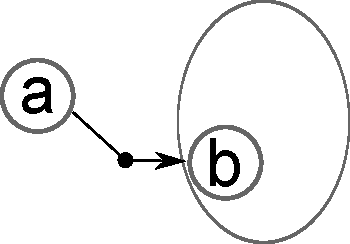
\includegraphics{./Figures/fig_exemplo.pdf}
	\end{center}
	\legend{Fonte: \citeonline[p.~12]{meregali}}
\end{figure}

\section{Descrição das Tabelas}
Veja exemplo de formatação da \autoref{tab:exemplo} a seguir: a legenda aparece
acima da tabela, à descrição deve ser centralizada, no número de identificação
2.1, o número 2 corresponde ao capítulo onde se localiza a tabela e o número 1
a ordem da tabela dentro do capítulo, seguido de travessão, espaço e título da
mesma, que deve ter a primeira letra em maiúsculo e o restante em minúsculo.

Observe que as laterais das tabelas são abertas. Isso torna a imagem mais limpa
e clara. As tabelas do texto não devem exceder a margem.

Em relação à referência da tabela, esta deve se localizar na parte inferior da
tabela, precedida da palavra fonte e seguida por dois pontos. Na sequência,
coloca-se o(s) nome(s) da(s) autoria(s) da tabela, seguida do ano e respectiva
página entre parênteses. Exemplo da \autoref{tab:exemplo}:

\begin{table}[htb]
	\centering
		\caption{Exemplo de apresentação de uma tabela no texto}
		\label{tab:exemplo}
		\begin{tabularx}{12cm}{>{\centering}X>{\centering}X X<{\centering}}
		\toprule
			\emph{Manga} & \emph{Abacaxi} & \emph{Morango} \\ \midrule
			12           & 100.000,00     & 10.000,00      \\
			12           & 10.000,00      & 100.000,00     \\ \bottomrule
		\end{tabularx}
		\legend{Fonte: \citeonline[p.~12]{meregali}}
\end{table}

%%%%%%%%%%%%%%%%%%%%%%%%%%%%%%%%%%%%%%%%%%%%%%%%%%%%%%%%%%%%%%

\chapter{Citações}
Há duas formas de se fazer uma citação: a \textbf{citação indireta} ou
\textbf{livre} (também chamada de paráfrase) e a \textbf{citação direta} ou
\textbf{textual}. Pode haver, ainda, a \textbf{citação de citação}. Todas as
citações devem trazer a identificação de sua autoria.

\section{Citação Indireta} A citação indireta ou livre (paráfrase) é aquela
citação na qual se expressa o pensamento de outra pessoa com nossas próprias
palavras. Após fazer a citação, deve-se indicar o nome do autor em letras
minúsculas se estiver no corpo do texto, e com letras maiúsculas se estiver
dentro dos parênteses, juntamente com o ano da publicação da obra em que se
encontra a ideia referida. Não são indicadas páginas já que a ideia pode estar
resumida de uma obra inteira, de um capítulo, de diversas partes ou de um
conjunto delas. Desta forma (com o nome no corpo do texto):

%%% OBS: os framed fazem parte do exemplo, e não devem aparecer no documento final
\begin{framed}
    Depois de analisar a situação, \citeonline{novoa1993} chegou a
    afirmar que o brasileiro ainda não está capacitado para escolher sua
    governante por causa de sua precária vocação política e da absoluta falta
    de escolaridade, já que o homem do povo, o zé-povinho, geralmente não sabe
    sequer em quem votou nas últimas eleições, não sabe sequer quem são seus
    governantes, não saber sequer quem determina seu próprio meio de
    sobreviver.
\end{framed}

Ou, então, com o nome nos parênteses:

\begin{framed}
    Depois de analisar a situação, chegou-se a afirmar que o brasileiro ainda
    não está capacitado para escolher sua governante por causa de sua precária
    vocação política e da absoluta falta de escolaridade, já que o homem do
    povo, o zé-povinho, geralmente não sabe sequer em quem votou nas últimas
    eleições, não sabe sequer quem são seus governantes, não saber sequer quem
    determina seu próprio meio de sobreviver \cite{novoa1993}.
\end{framed}

No caso de o autor possuir outras obras, elas serão diferenciadas pela data da
publicação.  Havendo mais de uma obra no mesmo ano, acrescentamos uma letra
após a data:

\begin{framed}
    No caso do teatro ou do cinema quem melhor se definiu foi
    \citeonline{antunes1997a} quando declarou que aqueles espaços haviam sido
    todos tomados pela geração de 40. Por outro lado, ele próprio se
    contradisse mais tarde (\citeyear{antunes1997b}).
\end{framed}

\section{Citação Direta}
São chamadas de citações diretas ou textuais aquelas em que se transcrevem
exatamente as palavras do autor citado. As citações diretas ou textuais podem
ser breves ou longas. São consideradas breves aquelas cuja extensão não
ultrapassa três linhas. Essas citações devem integrar o texto e devem vir entre
aspas. O tamanho da fonte da citação breve permanece o mesmo do corpo do texto.

\begin{framed}
    Vimos que, para nosso esclarecimento, precisamos seguir os preceitos
    encontrados, já que Guimarães estabelece: ``A valorização da palavra pela
    palavra encarna o objetivo precípuo do texto literário''
    (\citeyear{guim1985}, p.~32) e, se isso não ficar bem esclarecido, nosso
    trabalho será seriamente prejudicado.
\end{framed}

Ou assim:

\begin{framed}
    Vimos que, para nosso esclarecimento, precisamos seguir os preceitos
    encontrados, já que ficou estabelecido que ``A valorização da palavra pela
    palavra encarna o objetivo precípuo do texto literário''
    \cite[p.~32]{guim1985} e, se isso não ficar bem esclarecido, nosso trabalho
    será seriamente prejudicado.
\end{framed}

As citações com mais de três linhas são chamadas de longas e devem receber um
destaque especial com recuo de 4 cm da margem esquerda. Elas não deverão ter
aspas e o tamanho da fonte deve ser menor que o do texto (tamanho 10). A
distância entre as linhas do corpo da citação deve ser de um espaço simples.
Entre o texto da citação e o restante do trabalho, devem-se deixar dois espaços
1,5 cm antes e depois. Exemplo:

\begin{quote}
    Os pronomes O, A, OS e AS passam a serem pronomes demonstrativos sempre que
    numa frase puderem ser substituídos, sem alterar a estrutura dessa frase
    com toda certeza para facilitar a escrita na língua vernácula do próprio
    autor que pensou no seu público de origem. \cite[p.~19]{simoes}
\end{quote}

Havendo supressão de trechos no texto citado, faz-se a indicação com
reticências entre colchetes, denominadas elipses [...]: "Na comunicação diária,
aquela comunicação que utilizamos no dia-a-dia, além da referencialidade da
linguagem [...] há pinceladas de função conativa [...]" \cite[p.~37]{chalhub}.

Em relação à citação de uma citação, é a reprodução de uma informação já citada
por outro autor e, por sua vez, utiliza-se somente na impossibilidade de
consultar o documento original. No texto, deve ser citado o sobrenome do autor
do documento não consultado, seguido da expressão \textbf{apud}, e o nome do
autor do documento consultado. Em nota de rodapé devem ser mencionados os dados
do documento original. Na lista de referências bibliográficas, incluir o
documento efetivamente consultado. Outra opção é incluir as duas referências
dos documentos na lista de referências do trabalho; neste caso, não se inclui
nota de rodapé. A seguir um exemplo com nota de rodapé:


\begin{framed}
	Segundo \apudonline[ p.~5]{franco}{furtado}, texto texto texto texto texto
\end{framed}

ou

\begin{framed}
	texto texto texto texto texto \apud[ p.~5]{franco}{furtado}
\end{framed}